
%(BEGIN_QUESTION)
% Copyright 2006, Tony R. Kuphaldt, released under the Creative Commons Attribution License (v 1.0)
% This means you may do almost anything with this work of mine, so long as you give me proper credit

Bruk Bernoulli's formel for å regne ut trykket $P_2$. Massetettheten til fluidet er $\rho = 800kg/m$

%Use Bernoulli's equation to calculate the pressure at the throat of this ``venturi'' tube, assuming water flowing at a rate of 200 liter per sekund, with a weight density ($\gamma$) of 62.4 lb/ft$^{3}$ and a mass density ($\rho$) of 1.951 slugs/ft$^{3}$:

$$\includegraphics[width=15.5cm]{i00452x01.eps}$$

Bernoulli's formel:

\vskip 10pt

$$z_1 \rho g + {v_1^2 \rho \over 2} + P_1 = z_2 \rho g + {v_2^2 \rho \over 2} + P_2$$


\noindent
Where,

$z$ = Height of fluid, in meter (m)

$\rho$ = Mass density of fluid, in kg per kubikkmeter (kg/m$^3$)

$g$ = Acceleration of gravity (9.81 m/s$^{2}$)

$v$ = Hastigheten til fluidet i meter per sekund (m/s)

$P$ = Trykket av fluidet i Pascal (Pa=N/m²) 

\vskip 10pt

Til slutt regn ut differansetrykket i dette venturi måleelementet. ($\Delta P$)

\vskip 10pt

\vskip 20pt \vbox{\hrule \hbox{\strut \vrule{} {\bf Suggestions for Socratic discussion} \vrule} \hrule}

\begin{itemize}
\item{} The textbook outlines a general strategy for generating a problem-solving plan when tackling problems with complex mathematical formulae.  Specifically, this strategy involved writing out the formulae and linking variables between formulae with arrow symbols.  Explain how this strategy works, and show how it may be applied to the solution of this problem.
\item{} A very helpful strategy for tackling Bernoulli's equation problems is to create a table in which to place each of the ``head'' terms of that equation.  Explain why this is helpful to manage this specific type of problem.
\item{} Once we know the velocity of the fluid ($v$) at any point in the tube, is there a way to easily solve for the velocity in any other point in the tube based on a ratio of tube diameters?  For instance, here we know there is a 5:12 ratio of diameters from the throat to the mouth of the tube.  How can we employ this 5:12 ratio to easily determine the velocity at one point (either mouth or throat) knowing the velocity at another?
\end{itemize}

\underbar{file i00452}
%(END_QUESTION)





%(BEGIN_ANSWER)

$P_2$ = 0.43 MPa     

\vskip 10pt


Follow-up question: calculate the {\it differential} pressure between either $P_1$ or $P_3$ and $P_2$.

%(END_ANSWER)





%(BEGIN_NOTES)

% No blank lines allowed between lines of an \halign structure!
% I use comments (%) instead, so Tex doesn't choke.

$$\vbox{\offinterlineskip
\halign{\strut
\vrule \quad\hfil # \ \hfil & 
\vrule \quad\hfil # \ \hfil & 
\vrule \quad\hfil # \ \hfil \vrule \cr
\noalign{\hrule}
%
% First row
{\bf Head} & {\bf Calculation} at 12 inch tube & {\bf Value} \cr
%
\noalign{\hrule}
%
% Another row
$z_1 \rho g$ & (0 ft) (1.951 slugs/ft$^{3}$) (32.2 ft/s$^{2}$) & 0 lb/ft$^{2}$ \cr
%
\noalign{\hrule}
%
% Another row
$v_1^2 \rho / 2$ & (9.549 ft/s)$^{2}$ (1.951 slugs/ft$^{3}$) / 2 & 88.955 lb/ft$^{2}$ \cr
%
\noalign{\hrule}
%
% Another row
$P_1$ & (80 lb/in$^{2}$) (144 in$^{2}$/1 ft$^{2}$) & 11520 lb/ft$^{2}$ \cr
%
\noalign{\hrule}
%
% Another row
{\bf Total} &  0 lb/ft$^{2}$ + 88.955 lb/ft$^{2}$ + 11520 lb/ft$^{2}$ & {\bf 11608.955 lb/ft$^{2}$} \cr
%
\noalign{\hrule}
} % End of \halign 
}$$ % End of \vbox

\vskip 10pt

% No blank lines allowed between lines of an \halign structure!
% I use comments (%) instead, so Tex doesn't choke.

$$\vbox{\offinterlineskip
\halign{\strut
\vrule \quad\hfil # \ \hfil & 
\vrule \quad\hfil # \ \hfil & 
\vrule \quad\hfil # \ \hfil \vrule \cr
\noalign{\hrule}
%
% First row
{\bf Head} & {\bf Calculation} at 5 inch tube & {\bf Value} \cr
%
\noalign{\hrule}
%
% Another row
$z_2 \rho g$ & (0 ft) (1.951 slugs/ft$^{3}$) (32.2 ft/s$^{2}$) & 0 lb/ft$^{2}$ \cr
%
\noalign{\hrule}
%
% Another row
$v_2^2 \rho / 2$ & (55.004 ft/s)$^{2}$ (1.951 slugs/ft$^{3}$) / 2 & 2951.31 lb/ft$^{2}$ \cr
%
\noalign{\hrule}
%
% Another row
$P_2$ & (?? lb/in$^{2}$) (144 in$^{2}$/1 ft$^{2}$) & ??? lb/ft$^{2}$ \cr
%
\noalign{\hrule}
%
% Another row
{\bf Total} &  0 lb/ft$^{2}$ + 2951.31 lb/ft$^{2}$ + ??? lb/ft$^{2}$ & {\bf 11608.955 lb/ft$^{2}$} \cr
%
\noalign{\hrule}
} % End of \halign 
}$$ % End of \vbox

$$P_2 = 11608.955 \hbox{ lb/ft}^2 - 2951.31 \hbox{ lb/ft}^2 = 8657.64 \hbox{ lb/ft}^2 = 60.123 \hbox{ PSI}$$

\vskip 10pt

$\Delta P$ = $P_1 - P_2$ = 80 PSI $-$ 60.123 PSI = 19.877 PSI

\vskip 10pt

An interesting exercise is to double the flow rate and re-calculate the $\Delta P$.  You will see that this relationship is quadratic: doubling the flow quadruples the differential pressure.

%INDEX% Physics, dynamic fluids: Bernoulli's equation

%(END_NOTES)


